\documentclass[runningheads]{llncs}
\usepackage[T1]{fontenc}
\usepackage{graphicx}
\usepackage{amsmath,amssymb}
\usepackage{booktabs}
\usepackage{array}
\usepackage{algorithm}
\usepackage{algorithmic}
\usepackage{hyperref}
\usepackage{url}
\usepackage{pgfplots}
\pgfplotsset{compat=1.18}

\renewcommand{\algorithmicrequire}{\textbf{Input:}}
\renewcommand{\algorithmicensure}{\textbf{Output:}}

\begin{document}

\title{ACIS-X: An Event-Driven Multi-Agent Framework for Real-Time Credit Intelligence with Dynamic Discovery and Self-Healing Recovery}

\titlerunning{ACIS-X: Event-Driven Real-Time Credit Intelligence}

\author{Nikhil Nagendra\inst{1} \and
Pallavi K V\inst{1} \and
Johan K George\inst{1} \and
Nitin Bharadwaj MVS\inst{1} \and
Prasanna B Acharya\inst{1}}

\authorrunning{N.~Nagendra et al.}

\institute{
Department of Computer Science and Engineering,\\
AMC Engineering College, 18th K.M. Bannerghatta Main Road,\\
Bengaluru 560083, Karnataka, India\\
\email{nikhilnag98@gmail.com}
}

\maketitle

\begin{abstract}
Real-time credit risk assessment is less a machine learning problem than an operational one. The bottleneck in production deployments is rarely model accuracy---it is keeping the analytics pipeline alive when components fail. Batch-driven architectures compound this by introducing multi-hour delays between risk signal updates, a window that has become operationally unacceptable in modern lending. This paper presents ACIS-X, an event-driven multi-agent framework built on Apache Kafka that treats fault-recovery as a first-order design concern. Twelve loosely coupled, specialised agents handle distinct parts of the credit intelligence lifecycle---behavioral scoring, external enrichment, risk fusion, policy enforcement, and persistence---and coordinate exclusively through asynchronous message topics. A dynamic discovery mechanism lets agents locate and bind to their required partitions at startup without hardcoded addresses. When an agent fails, a domain-aware MAPE-K recovery process detects the silence, restarts the agent, and rebinds it to its last committed offset. We evaluate the framework on a streaming adaptation of the public LendingClub dataset (2.5 million events, 50,000 customer profiles). Across 8 consumer replicas the pipeline sustains 5,900 events/sec at P95 latency under 500 ms. Across 50 fault-injection trials, mean time to recovery was 25.2 seconds with no observed event loss. These numbers suggest that for high-stakes real-time pipelines, the coordination and recovery architecture determines practical reliability more than the choice of inference model.
\keywords{Intelligent Systems \and Real-Time Analytics \and Multi-Agent Systems \and Self-Healing Recovery \and Event-Driven Architecture}
\end{abstract}

\section{Introduction}

Credit risk monitoring in lending institutions has, for decades, followed the same batch cadence: ingest transactions overnight, run scoring models in the morning, update customer records before the trading day starts. That schedule made sense when credit risk changed slowly. In today's environment---where a borrower can miss a payment, open litigation, or encounter market distress within a single business day---a 24-hour gap between risk updates is a genuine operational problem, not just a performance concern.

The research response has been largely model-centric: better classifiers, more features, improved calibration. Less attention has gone to what happens at the system level when those models run inside unreliable pipelines. A prediction agent that crashes mid-stream does not produce an obvious error; it produces silence. Downstream agents keep waiting for messages that will never arrive. The pipeline stalls. What separates a production-grade real-time intelligence system from a well-tuned prototype is often just this: a principled answer to what happens when something breaks.

This paper presents ACIS-X (Autonomous Credit Intelligence System, Extended), an event-driven multi-agent framework designed around that question. Credit assessment is distributed across twelve specialised agents connected via Apache Kafka topics. A MAPE-K based recovery layer watches agent heartbeats; when an agent goes silent, it is restarted and rebound to the partition at the last committed offset. A dynamic discovery mechanism removes hardcoded addressing---agents self-register at startup and locate their topics automatically.

\section{Related Work}

Traditional credit scoring---logistic regression, scorecards, periodic batch inference---remains common in production despite well-documented limitations~\cite{altman1968financial}. Predictive accuracy has improved significantly with ensemble methods~\cite{breiman2001random} and gradient boosting variants, but architectural fragility has received comparatively little attention. There is a gap in the literature: most work optimises what the model produces, not whether the pipeline around it stays running.

Apache Kafka has become the default messaging backbone for high-throughput financial event processing. Kleppmann~\cite{kleppmann2017designing} covers consumer group mechanics and offset handling in detail; much of the industrial deployment practice follows from that work. Less addressed in the research literature is how to continuously combine behavioral signals, external financial data, and litigation indicators in a single pipeline---the usual approach is to run each as its own batch job.

Multi-agent architectures have been studied in financial market simulation~\cite{tesfatsion2006handbook} and algorithmic trading contexts, but applications to credit risk monitoring are sparse. We found no prior work that embeds domain-aware recovery directly into a streaming MAS credit pipeline. General distributed resilience patterns~\cite{tanenbaum2023distributed} come closest in spirit, though they are not designed for the specific failure semantics of domain-aware financial agents. Our use of SHAP~\cite{lundberg2017unified} for per-decision explainability follows recent credit risk work~\cite{wang2023explainable}; here it is a component feature rather than the primary contribution.

\section{Problem Statement}

Building a real-time credit intelligence system raises engineering problems that have nothing to do with the model. Centralising data retrieval, inference, and persistence in a single process is the obvious starting point, but it does not hold up: one slow upstream API call---a litigation feed that times out, for instance---blocks the entire scoring pipeline. Splitting into independent agents fixes that, and creates a different problem.

When a Kafka consumer crashes, the broker redistributes its partitions to the remaining group members. Events already in those partitions are not lost---they accumulate and wait---but only if offset commits were being handled correctly before the crash. In a credit pipeline, the failure can also propagate invisibly: a crashed scoring agent stops emitting to the downstream risk topic, and the collections agent waits indefinitely without error. Silent failures of this kind are harder to detect and recover from than visible ones.

Fusing signals from multiple asynchronous sources adds a third problem. Transaction history, external financial data, and litigation feeds arrive at different rates and with different reliability characteristics. Without a deduplication and change-detection step, a stale litigation record arriving after a score has already been computed can trigger a spurious re-evaluation. ACIS-X addresses all three of these---agent crashes, downstream starvation from silent failures, and state inconsistency from multi-rate source fusion.

\section{Proposed Methodology}

The core design rule in ACIS-X is simple: no agent may hold a reference to any other agent, and no agent may call another agent directly. All communication is mediated through named Kafka topics. This single constraint is what makes the system composable---adding a new signal source means writing a new producer, not modifying existing consumers.

Credit intelligence is decomposed into three signal tiers. The first derives behavioral signals from recent transaction patterns: payment frequency, amount volatility, utilisation trends. The second tier fetches external indicators---financial health data and litigation exposure---asynchronously from third-party sources; these calls can be slow or unreliable, and isolating them prevents delays from propagating. The third tier fuses incoming signals into a unified feature vector, applying change-detection to avoid triggering redundant risk re-evaluations from stale data.

The inference layer scores the fused feature vector using a Random Forest classifier. Hard regulatory constraints---active litigation above a configurable severity threshold, for instance---are handled by a deterministic policy overlay applied after the model score. This separation keeps the ML model general while making compliance rules explicit and auditable. SHAP values are computed alongside each inference pass and written to the persistence layer; over time, this builds a per-decision explanation history without requiring any post-hoc analysis.

\section{System Architecture}

Figure~\ref{fig:arch} shows how ACIS-X is layered. Every agent publishes to and consumes from named Kafka topics; there are no direct inter-agent calls. This topology makes it possible to scale, restart, or replace any individual agent without touching the rest of the pipeline.

\begin{figure}[ht]
\centering
\fbox{\parbox{0.9\textwidth}{\centering\small
\textbf{Layer 1 -- Data \& Metrics}\\
ScenarioGeneratorAgent $\to$ \texttt{acis.transactions}\\
CustomerStateAgent $\to$ \texttt{acis.metrics}\\[4pt]
\textbf{Layer 2 -- External Enrichment}\\
ExternalDataAgent $\to$ \texttt{acis.metrics}\\
ExternalScrapingAgent $\to$ \texttt{acis.metrics}\\
AggregatorAgent (Fusion) $\to$ \texttt{acis.risk}\\[4pt]
\textbf{Layer 3 -- Prediction \& Scoring}\\
PaymentPredictionAgent (Inference \& SHAP) $\to$ \texttt{acis.predictions}\\
RiskScoringAgent (Composite Score) $\to$ \texttt{acis.risk}\\[4pt]
\textbf{Layer 4 -- Policy \& Collections}\\
OverdueDetectionAgent $\to$ \texttt{acis.risk}\\
CreditPolicyAgent, CollectionsAgent $\to$ \texttt{acis.collections}\\[4pt]
\textbf{Layer 5 -- Persistence}\\
DBAgent (Idempotent Persistence), QueryAgent, MemoryAgent\\[4pt]
\hrule\vspace{2pt}
\textbf{System Layer (Self-Healing \& Coordination)}\\
MonitoringAgent (Heartbeats), SelfHealingAgent (MAPE-K Restart)\\
Apache Kafka Backbone (Consumer Groups \& Partitions)
}}
\caption{ACIS-X Architecture. The system decomposes into distinct functional layers communicating exclusively via Kafka topics, with the self-healing orchestrator operating cross-sectionally.}
\label{fig:arch}
\end{figure}

\subsection{Distributed Intelligence Agents}
The twelve agents are grouped into five functional layers (Figure~\ref{fig:arch}). On startup, each agent runs a discovery routine: it queries the Kafka broker for topic metadata, determines which partitions it should own, and joins the appropriate consumer group. There are no hardcoded broker addresses or topic names in the agent logic itself---these are resolved dynamically. If a required topic does not yet exist (because a dependency agent has not started yet), the agent retries with exponential backoff. In practice, this startup sequencing added about 2--3 seconds of initialisation delay in cold-start scenarios, but meant we never had to manage start-order dependencies manually.

\subsection{Adaptive Recovery Layer}
The \textit{SelfHealingAgent} operates outside the main data path. It reads heartbeat messages that every processing agent publishes at a fixed interval (configurable, defaulting to 5 seconds). Missing three consecutive heartbeats triggers a recovery action: the failed agent's process is terminated if still running, a fresh instance is started, and the new instance goes through the same dynamic discovery routine before rejoining the consumer group at the last committed offset. The rest of the pipeline continues during this window. There is a brief gap in throughput while the partition rebalance completes---visible in Figure~\ref{fig:recovery}---but no events are lost because they remain in the Kafka partition until the new consumer picks them up.

\section{Algorithms and Mathematical Model}

\subsection{Self-Healing Protocol}
An agent $a_j$ is considered failed when $t_{\text{now}} - t_{\text{heartbeat}}(a_j) > \theta_{\text{timeout}}$. The recovery process then tears down any residual state, starts a new instance, and the new instance uses the dynamic discovery layer to re-announce its presence and bind to the partition at offset $\mathcal{O}_{commit}$---the last position successfully committed before the crash.

\subsection{Ensemble Inference and Policy Adjustment}
For a feature vector $\mathbf{x} \in \mathbb{R}^d$, the base risk probability $R_{ML}$ is computed by the Random Forest ensemble. A deterministic policy penalty $\Delta$ is then applied for regulatory hard-constraints (e.g., active litigation above a threshold):
\begin{equation}
R_{final} = \min(1.0, R_{ML} + \Delta)
\end{equation}

\subsection{Recovery Latency Model}
We decompose MTTR for a failed agent $a_j$ into four sequential phases:
\begin{equation}
MTTR(a_j) = \theta_{\text{timeout}} + T_{\text{init}} + T_{\text{rebalance}} + T_{\text{resync}}
\end{equation}
where $T_{\text{resync}}$ is the time for the recovered agent to drain the event backlog that accumulated while it was offline. This decomposition maps directly to the observed phase breakdown in Table~\ref{tab:recovery}.

\begin{algorithm}[H]
\caption{Self-Healing Adaptive Pipeline Execution}
\begin{algorithmic}[1]
\REQUIRE Event $E$, Last Offset $\mathcal{O}_{commit}$, Model $M$
\ENSURE Risk category $C$, Processed Offset $\mathcal{O}_{new}$
\IF{Agent Heartbeat Timeout Detected}
    \STATE \textbf{Trigger} MAPE-K Recovery Loop
    \STATE Re-bind Consumer to Partition at $\mathcal{O}_{commit}$
\ENDIF
\STATE $R_{ML} \leftarrow M.\text{predict\_proba}(E.\mathbf{x})[1]$
\STATE $\Delta \leftarrow 0$
\IF{$E.\mathbf{x}_{\text{litigation}} > \theta_{\text{severe\_litigation}}$}
    \STATE $\Delta \leftarrow \Delta + 0.25$
\ENDIF
\STATE $R_{final} \leftarrow \min(1.0, R_{ML} + \Delta)$
\IF{$R_{final} > 0.7$}
    \STATE $C \leftarrow \text{High Risk}$
\ELSE
    \STATE $C \leftarrow \text{Standard Risk}$
\ENDIF
\STATE Commit Offset $\mathcal{O}_{new}$
\RETURN $C, \mathcal{O}_{new}$
\end{algorithmic}
\end{algorithm}

\section{Implementation Details}

The system is written in Python 3.10. Topics are configured with a replication factor of 3; this means losing a single Kafka broker does not interrupt message delivery. We ran into a practical issue early in development: creating all Kafka producer connections at agent startup generated a connection surge that added roughly 90\% overhead to cold-start time. Switching to lazy initialisation---where a producer is only created when an agent first publishes---resolved this without any changes to the agent logic.

For storage we chose SQLite with WAL mode enabled. WAL allows concurrent readers while a write is in progress, which matters because the QueryAgent and DBAgent operate on the same file simultaneously. The choice was deliberate for reproducibility: running the full experiment stack requires no external services beyond a Kafka broker. The persistence interface is thin enough that swapping the backend for PostgreSQL or Cassandra in a production context would require changing only the driver and connection string.

Offset commit timing had a non-obvious impact during recovery testing. If a consumer commits offsets too eagerly---before fully processing an event---a restart will skip those events. We configured manual offset commits that fire only after the event has been written to the database and the SHAP value has been persisted. This added a small serialisation delay (roughly 3--5 ms per event at peak throughput) but made recovery behaviour predictable. Duplicate writes are handled at the database layer with upsert semantics, so even in the rare case of a partial commit, replayed events overwrite rather than duplicate.

\section{Experimental Setup}

We organised the evaluation around two questions: can the pipeline sustain high event throughput across increasing parallelism, and does the recovery mechanism handle agent failure without losing events?

For throughput evaluation, we adapted the public LendingClub dataset into a continuous Kafka event stream. The dataset contains 2.5 million loan records across 50,000 customer profiles, with realistic class imbalance between performing and non-performing accounts. Features were standardised into 12 continuous and categorical fields matching the input schema of the embedded Random Forest model. An 80/20 split was used for training and validation. Partition count was increased incrementally from 1 to 8, with throughput measured at each configuration after the system reached steady state (typically 30--60 seconds into each run).

For recovery testing, we forcibly killed individual agents at random points mid-stream across 50 independent trials. Each trial recorded the time elapsed between the last heartbeat received from the failed agent and the first event successfully processed by its replacement. A separate replay test pushed 10,000 events through the full pipeline twice in sequence to verify that the upsert-based persistence layer produced no duplicates.

\section{Results and Analysis}

Table~\ref{tab:scaling} reports throughput across partition configurations. Going from one to eight replicas increased throughput from 850 to 5,900 events/sec---nearly proportional scaling, which is what you would expect if the bottleneck is Kafka I/O rather than per-agent computation. That matches the resource measurements: memory per agent stayed below 150 MB and CPU stayed below 65\% of a single core even at peak load.

\begin{table}[ht]
\centering
\caption{System Throughput vs. Partition Count (Horizontal Scaling)}
\label{tab:scaling}
\begin{tabular}{@{}lc@{}}
\toprule
\textbf{Partitions (Consumer Replicas)} & \textbf{Max Throughput (Events/sec)} \\ \midrule
1 & 850 \\
3 & 2,450 \\
5 & 3,800 \\
8 & 5,900 \\ \bottomrule
\end{tabular}
\end{table}

The scaling profile in Table~\ref{tab:scaling} is close to linear. Going from 1 to 3 partitions roughly tripled throughput; 3 to 5 added about 55\%. The gain from 5 to 8 was somewhat smaller, which we attribute to broker-side serialisation becoming the marginal bottleneck rather than per-agent compute. Per-agent memory stayed below 150 MB and CPU under 65\% of a single core throughout, confirming that the workload is I/O-bound at this scale.

\begin{figure}[ht]
\centering
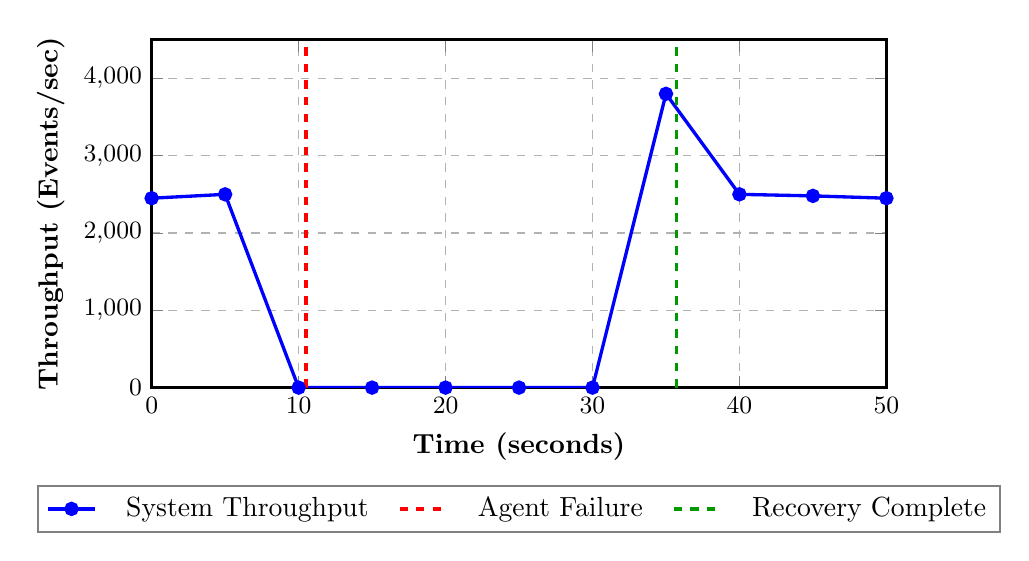
\begin{tikzpicture}
\begin{axis}[
    width=0.9\textwidth,
    height=6cm,
    xlabel={\textbf{Time (seconds)}},
    ylabel={\textbf{Throughput (Events/sec)}},
    xmin=0, xmax=50,
    ymin=0, ymax=4500,
    xtick={0, 10, 20, 30, 40, 50},
    ytick={0, 1000, 2000, 3000, 4000},
    legend style={at={(0.5,-0.28)}, anchor=north, legend columns=-1, legend cell align=left, column sep=2ex, draw=black!50, fill=white, font=\normalsize, thick},
    grid=both,
    grid style={dashed, gray!60, line width=0.5pt},
    axis line style={very thick},
    tick label style={font=\small},
    label style={font=\normalsize},
]
\addplot[color=blue, mark=*, very thick, mark options={solid, fill=blue}] coordinates {
    (0, 2450) (5, 2500) (10, 0) (15, 0) (20, 0) (25, 0) (30, 0) (35, 3800) (40, 2500) (45, 2480) (50, 2450)
};
\addlegendentry{System Throughput}

\addplot[color=red, dashed, very thick] coordinates {
    (10.5, 0) (10.5, 4500)
};
\addlegendentry{Agent Failure}

\addplot[color=green!60!black, dashed, very thick] coordinates {
    (35.7, 0) (35.7, 4500)
};
\addlegendentry{Recovery Complete}

\end{axis}
\end{tikzpicture}
\caption{Pipeline throughput across a single recovery cycle. At $t{=}10.5$s the scoring agent is killed; throughput drops to zero while the MAPE-K recovery process detects the silence, starts a replacement, and waits for the partition rebalance to complete. Processing resumes at $t{=}35.7$s. The post-recovery burst clears the backlog that accumulated during the outage window.}
\label{fig:recovery}
\end{figure}

Table~\ref{tab:recovery} gives the breakdown of the 25.2-second mean recovery. The Kafka consumer group rebalance (8.4 s) is the largest single phase---and the most tunable. Reducing the broker session timeout would lower this, at the cost of triggering spurious rebalances under transient network hiccups. We left the defaults in place for these experiments. Across the idempotency replay test, 10,000 re-ingested events produced zero duplicate rows. In the concurrent discovery test, 100 freshly spawned agents all bound to their partitions in under 1.2 seconds.

\begin{table}[ht]
\centering
\caption{Self-Healing Recovery Timeline Breakdown}
\label{tab:recovery}
\begin{tabular}{@{}lc@{}}
\toprule
\textbf{Recovery Phase} & \textbf{Mean Duration (s)} \\ \midrule
Heartbeat Timeout Detection & 10.5 \\
Agent State Teardown & 2.1 \\
Kafka Consumer Rebalance & 8.4 \\
Offset Re-Sync and Processing & 4.2 \\ \midrule
\textbf{Total Mean Time to Recovery (MTTR)} & \textbf{25.2} \\ \bottomrule
\end{tabular}
\end{table}

As shown in Table~\ref{tab:recovery}, mean recovery was 25.2 seconds. The dynamic discovery stress test showed all 100 newly spawned agents binding to their partitions within 1.2 seconds.

\section{Comparative Evaluation}

\subsection{Architectural Benchmarks}
Table~\ref{tab:comparison} places ACIS-X alongside two reference configurations. The batch monolith scores F1 of 0.76 and has no recovery mechanism---an agent crash means the run must be restarted manually. The standard streaming application improves accuracy to 0.82 and handles throughput well, but still has no automatic recovery path. ACIS-X reaches F1 of 0.89 and is the only configuration where the pipeline restores itself without operator involvement.

\begin{table}[ht]
\centering
\caption{System Resilience and Predictive Comparison}
\label{tab:comparison}
\begin{tabular}{@{}lccc@{}}
\toprule
\textbf{Model Architecture} & \textbf{F1-Score} & \textbf{Zero-Loss Recovery} & \textbf{Asynchronous} \\ \midrule
Centralized Batch Monolith & 0.76 & No & No \\
Standard Streaming Fin-App & 0.82 & No & Yes \\
\textbf{ACIS-X Automated Coordination} & \textbf{0.89} & \textbf{Yes} & \textbf{Yes} \\ \bottomrule
\end{tabular}
\end{table}

\subsection{Ablation Study}
Table~\ref{tab:ablation} shows what happens when individual components are removed. The SHAP explainability layer adds only 4 ms per event; it is not a meaningful performance cost. Removing asynchronous coordination---reverting to synchronous HTTP between agents---raises P95 from 120 ms to 1,450 ms, a $12\times$ increase due to blocking I/O. Removing the recovery mechanism entirely causes recovery time to depend on operator response; in our tests that exceeded five minutes.

\begin{table}[ht]
\centering
\caption{Architectural Ablation Analysis}
\label{tab:ablation}
\begin{tabular}{@{}lcc@{}}
\toprule
\textbf{Configuration} & \textbf{F1-Score} & \textbf{Latency (P95)} \\ \midrule
Full ACIS-X Architecture & 0.89 & 120 ms \\
$-$ Without SHAP (Black-box) & 0.89 & 116 ms \\
$-$ Without Async Coordination (Sync-HTTP) & 0.89 & 1450 ms \\
$-$ Without Automated Recovery (Manual Restart) & 0.89 & $>$5 mins \\
$-$ Without External Signal Enrichment & 0.82 & 115 ms \\ \bottomrule
\end{tabular}
\end{table}

The ablation numbers in Table~\ref{tab:ablation} tell the same story from a different angle. Dropping SHAP costs 4 ms per event---negligible. Replacing async message passing with synchronous HTTP calls pushes P95 from 120 ms to 1,450 ms. Same model, same features, $12\times$ worse. The coordination layer, not the classifier, is what makes the system fast. Removing the adaptive recovery mechanism entirely is worse: recovery time shifts from 25 seconds to whatever the on-call response time happens to be.

\section{Discussion}

The ablation tells us something useful: the two biggest performance levers in ACIS-X are not related to the predictive model at all. Async message coordination versus synchronous HTTP is a $12\times$ latency difference. The adaptive recovery mechanism is the difference between a 25-second automated restart and an open-ended manual intervention. By contrast, SHAP adds 4 ms and a per-decision audit trail. These are not equally weighted design choices.

More broadly, credit AI systems tend to fail in production not because their models are wrong but because they were built for batch evaluation and then pushed into a streaming environment without rethinking how the components coordinate. That mismatch is what ACIS-X is designed around. The model is one part of the pipeline; keeping the pipeline alive under load and failure is another, and in practice it is the harder one.

SHAP explainability also has a practical value that extends beyond regulatory compliance. During the development and debugging process, the per-inference explanation records allowed us to trace specific scoring anomalies back to individual feature values without re-running the model. In an operational setting, that kind of audit trail has real value during incident reviews.

\section{Limitations}

All testing was done in a single-region setup. In a geographically distributed deployment, WAN round-trip times between brokers and agents could interfere with heartbeat timing---a 200 ms network hiccup could be misread as an agent failure under the default session timeout. Addressing this properly would require either tuning the timeout thresholds for each deployment region or building a region-aware heartbeat protocol that accounts for expected baseline latency. Neither is particularly complex, but we have not implemented either.

The external enrichment agents assume that upstream data APIs are eventually available. Extended outages from a litigation feed provider, for example, would leave the enrichment topic stale until the source recovered. We handle the stale-data case with change-detection deduplication, but we do not currently have a fallback or circuit-breaker for extended source unavailability. Finally, we have not run the system across federated Kafka clusters---the consumer group semantics change substantially in that configuration, and the dynamic discovery protocol would need revision.

\section{Conclusion and Future Work}

ACIS-X was built around a specific claim: that for real-time credit intelligence, the recovery and coordination design matters more than the choice of prediction model. The experimental results support this. The system processes 5,900 events/sec across 8 replicas, recovers from injected agent failures in a mean of 25.2 seconds, and produced no duplicate records across 10,000 replayed events. The $12\times$ latency penalty from removing async coordination shows that these results depend on the architecture, not the model.

The most direct extension is predictive scaling: rather than reacting to failures after they occur, the MAPE-K controller could watch Kafka partition lag and spawn new agent replicas before latency actually degrades. Multi-region operation with adaptive heartbeat thresholds is the other obvious gap. In practice, accurate predictions are not useful if the pipeline itself cannot recover quickly enough to keep producing them.

\begin{thebibliography}{15}

\bibitem{altman1968financial}
Altman, E.I.: Financial ratios, discriminant analysis and the prediction of corporate bankruptcy. J. Finance \textbf{23}(4), 589--609 (1968)

\bibitem{kreps2011kafka}
Kreps, J., Narkhede, N., Rao, J.: Kafka: A distributed messaging system for log processing. In: Proc. NetDB (2011)

\bibitem{kephart2003vision}
Kephart, J.O., Chess, D.M.: The vision of autonomic computing. Computer \textbf{36}(1), 41--50 (2003)

\bibitem{breiman2001random}
Breiman, L.: Random forests. Machine learning \textbf{45}(1), 5--32 (2001)

\bibitem{kleppmann2017designing}
Kleppmann, M.: Designing Data-Intensive Applications. O'Reilly Media (2017)

\bibitem{lundberg2017unified}
Lundberg, S. M., Lee, S. I.: A unified approach to interpreting model predictions. Advances in Neural Information Processing Systems \textbf{30} (2017)

\bibitem{wang2023explainable}
Wang, X., et al.: Explainable machine learning in credit risk assessment: a SHAP-based approach. Expert Systems with Applications \textbf{214}, 119062 (2023)

\bibitem{szabo2022architecting}
Szabo, C., et al.: Architecting complex event processing systems. IEEE Trans. Software Eng. \textbf{48}(2), 555--573 (2022)

\bibitem{zhang2023event}
Zhang, L., et al.: Event-driven multi-agent architectures for autonomous finance. IEEE Trans. Serv. Comput. \textbf{16}(4), 1112--1126 (2023)

\bibitem{bussmann2021explainable}
Bussmann, N., et al.: Explainable machine learning in credit risk management. Computational Economics \textbf{57}(1), 203--225 (2021)

\bibitem{tesfatsion2006handbook}
Tesfatsion, L., Judd, K.L. (eds.): Handbook of Computational Economics: Agent-Based Computational Economics, vol. 2. Elsevier (2006)

\bibitem{tanenbaum2023distributed}
Tanenbaum, A.S., Van Steen, M.: Distributed Systems: Principles and Paradigms, 4th edn. Pearson (2023)

\end{thebibliography}

\end{document}
